\chapter{Evaluierung Permissioned Blockchains für B2B}
\label{cha:b2b-eval}

Die Blockchain-Technologie bringt diverse Probleme mit sich, welche je nach Anwendungszweck und Blockchaintyp verschieden große Auswirkungen haben. Für den B2B-Bereich gilt es vor allem die Skalierbarkeit sowie die Konsensmechanismen zu analysieren.

\section{Skalierbarkeit}
\label{sec:scalability-eval}
Das CAP-Theorem besagt, dass es in einem verteilten System nur möglich ist, 2 von den 3 folgenden Eigenschaften zu erfüllen: Konsistenz, Verfügbarkeit und Ausfalltoleranz. Bei der Blockchain wären dies: Dezentralisierung, Skalierbarkeit und Nichtangreifbarkeit \cite{SchererPerformanceScalabilityBlockchain2017}. Im Bezug auf die Skalierbarkeit wird vor allem auf den Transaktionsdurchsatz sowie die Bestätigungszeiten von Transaktionen eingegangen. Dazu erfolgt zunächst eine Analyse an aktuellen Public Blockchains, und letztendlich an Permissioned Blockchains. Die Ergebnisse werden ebenfalls auf das CAP-Theorem angewandt.  

\subsection{Public Blockchains}

\begin{figure}[htb]
  \centering
    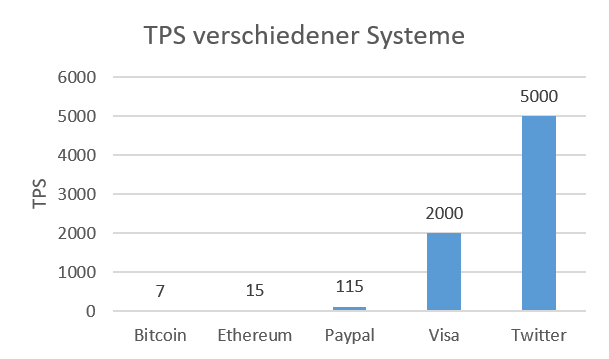
\includegraphics[width=0.9\textwidth,angle=0]{images/tps-comparison}
     \caption{Möglicher Transaktionsdurchsatz bei Bitcoin, Ethereum, Paypal und Visa \cite{BitcoinTeamScalabilityBitcoinWiki}.}
    \label{fig:tps-comparison}
\end{figure}

%TODO: Bitcoin-Kapitel nochmal unterteilem in paragraphs ?
\subsubsection{Bitcoin}
%TODO: Transaktionsgebühren erwähnen ?
Das Bitcoin-Netzwerk erreicht aktuell einen maximalen Transaktionsdurchsatz von 7 Transaktionen (Unterschiedlich je nach Größe der Transaktionen) pro Sekunde (TPS), bei einer Blockgröße von 1MB.  Hingegen erreicht Paypal 115 TPS, und Visa 2000 TPS (Siehe auch Abb. \ref{fig:tps-comparison}) \cite{BitcoinTeamScalabilityBitcoinWiki}. Hinzu kommt, dass ungefähr 170000 unbestätigte Transaktionen\footnote{Unbestätigte Transaktion: Eine Transaktion, welche noch nicht in einen Block vorkommt \cite{AntonopoulosMasteringbitcoin2015}.} bestehen \cite{BlockchainUnternehmenUnbestatigteTransaktionenBitcoin}. Berechnungen von Scherer zeigen, dass bei 11,8 Millionen Nutzern im Bitcoin-Netzwerk, sowie einem Transaktionsdurchsatz von 4 TPS, jeder Nutzer nur nur ca. 10 Transaktionen im Jahr senden kann \cite{SchererPerformanceScalabilityBlockchain2017}.

%TODO: SegWit ?
Der Transaktionsdurchsatz ist durch verschiedene Faktoren limitiert. Hauptsächlich durch die limitierte Blockgröße von 1MB, und dem PoW: Nur eine bestimmte Anzahl an Transaktionen passt in einen Block, und nur alle 10 Minuten wird einer erstellt. Es gäbe also die Möglichkeit, die Blockgröße zu vergrößern, oder die Zeit für den PoW zu verringern, indem die Schwierigkeit angepasst wird. Es gibt jedoch diverse Nachteile, welche dadurch entstehen würden. Bei einer größeren Blockgröße würde es länger dauern, bis ein Block beim Propagieren durch das Netzwerk alle Nodes erreicht. Dies würde zu öfter vorkommenden und längeren Forks führen und somit die Sicherheit des Netzwerks beeinträchtigen. Den gleichen Effekt hätte eine kürzere PoW Zeit, da die Wahrscheinlichkeit höher ist, dass zwei Nodes zur ungefähr gleichen Zeit einen Block erstellen \cite{SchererPerformanceScalabilityBlockchain2017} \cite{EthereumTeamEthereumWhitePaper2017} \cite{SompolinskyAcceleratingBitcoinTransaction2013}. 

Entsteht ein Fork, probieren Nodes die längere und somit gültige Blockchain zu erschaffen. Gelingt dies, wird die kürzere Blockchain mit den nun sogenannten Stale Blocks verworfen. Die gesamte Rechenleistung, welche in die Stale Blocks und seine Nachfolger geflossen ist, trägt nicht zur Sicherheit des Netzwerks bei. Dies lässt sich auch anhand der Abbildung \ref{fig:forking-risks} erläutern. Innerhalb der Blockchain bestehen durch mehrere Forks 5 Branches. Das bedeutet, dass die Rechenleistung des Netzwerks auf diese aufgespalten ist. Es wird davon ausgegangen, dass 20\% der Rechenleistung in den obersten Branch geflossen ist, welcher der längste ist. Die restlichen 4 Branches erhalten je 10\% der Rechenleistung. Wenn es nun einen Angreifer mit 40\% der Rechenleistung probiert eine eigene Blockchain zu erstellen, gelingt ihm dies, da er schneller die längere Blockchain erstellen kann \cite{SompolinskyAcceleratingBitcoinTransaction2013}. Zusammenfassend lässt sich sagen, dass ein Angreifer nicht 51\% der Rechenleistung für einen Fork benötigt, wenn das Netzwerk diese bei Forks verschwendet \cite{Buterin12secondBlockTime2014}. 

Ein weiteres Problem der Forks ist, dass Miner keine Belohnung für die Arbeit an verworfenen Blöcken erhalten. Dadurch kann es zur Zentralisierung durch wachsende Mining Pools kommen. Dies wird an folgenden Beispiel ersichtlich: Ein Mining Pool A besitzt 30\% der Rechenleistung, ein Mining Pool B 10\%. In dem genannten Beispiel würde Mining Pool A in 70\% aller Fälle einen Stale Block erzeugen, und B in 90\% aller Fälle. Kein Miner würde dem Mining Pool B beitreten, da die Wahrscheinlichkeit geringer ist, dass B gültige Blöcke erschafft. A hingegen würde immer mehr Miner, und somit mehr Rechenleistung erhalten \cite{EthereumTeamEthereumWhitePaper2017}.

%TODO: Quelle
%TODO: Benachteiligung von Minern erwähen ?
%Ein weiterer wichtiger Punkt in Bezug auf die Propagationszeiten ist die Benachteiligung von Minern.  Nodes, welche neue Blöcke erst später erhalten, können erst später mit dem Mining beginnen. Dazu ein Beispiel: Ein Miner A besitzt 45\% der Rechenleistung und es dauert 4 Sekunden bis ein Block bei allen anderen Nodes angekommen ist. Alle 5 Sekunden entsteht ein neuer Block. A wird in 45\% aller Fälle einen Block an die Blockchain anhängen. Er kann direkt mit den minen des neuen Blocks anfangen, während alle anderen Nodes erst nach 4 Sekunden erfahren, dass bereits ein neuer Block gefunden wurde. Alle anderen Nodes hätten somit nur noch 1 Sekunde um einen neuen Block an diesen anzuhängen. Somit würde hauptsächlich A Blöcke erstellen, und damit die Kontrolle über das Netzwerk haben.

An dieser Stelle sollte auch darauf hingewiesen werden, dass schnellere Blockerstellungszeiten nicht zwingend zu schnelleren Transaktionsbetätigungen führen. Transaktionen werden zwar schneller in Blöcken aufgenommen, aber es muss auf mehr Nachfolger gewartet werden, um sicher zu gehen, dass die Transaktion nicht in einem Fork vorkommt \cite{SchererPerformanceScalabilityBlockchain2017}.

\subsection{Ethereum}

\paragraph{Bessere Skalierbarkeit durch GHOST}
Das Ethereum Netzwerk nutzt das sogenannte GHOST-Protokoll, und erreicht damit eine Transaktionsdurchsatz von 15 TPS, bei einer durchschnittlichen Zeit von 15 Sekunden um den PoW zu erbringen. Dieses löst Probleme des Forkings und der Benachteiligung von Minern. Ersteres wird dadurch gelöst, dass Stale Blocks in die Berechnung der gültigen Blockchain einfließen. Anders als bei Bitcoin, wo lediglich die Parents und deren Nachfolger eine Rolle spielen. Die Stale Blocks werden in Ethereum ``Uncles'' genannt. Kurz gesagt, ist ein Uncle ein alternativer gefundener Block welcher auf der gleichen Höhe wie der Parent bestehen würde \cite{EthereumTeamEthereumWhitePaper2017}.

Die Bestimmung der gültigen Blockchain wird an der Abbildung \ref{fig:forking-risks} ersichtlich. In Ethereum ist die Blockchain die gültige, für welche die meiste Arbeit aufgebracht wurde, unter Einbezug der Uncles. Das führt dazu, dass der Branch mit den meisten Uncles bestehen bleibt. Das bedeutet letztendlich, dass die gesamte Rechenleistung das Netzwerk absichert, auch wenn diese sich auf die Branches aufteilt. Ein Angreifer braucht somit weiterhin 51\% der Rechenleistung um einen Angriff auszuführen \cite{SompolinskyAcceleratingBitcoinTransaction2013}.

Damit ist allerdings noch nicht das Problem der Zentralisierung durch Mining Pools gelöst. Es besteht weiterhin keine Motivation für Miner, Uncles zu minen. Deswegen ist das GHOST-Protokoll in Ethereum so erweitert, dass Miner Ether\footnote{Kryptowährung von Ethereum \cite{EthereumTeamEthereumWhitePaper2017}.} als Belohnung für das Erstellen von Uncles erhalten (Allerdings weniger als bei vollwertigen Blöcken). Somit besteht ebenfalls die Motivation, kleineren Mining Pools beizutreten \cite{EthereumTeamEthereumWhitePaper2017}. An dieser Stelle sollte auch erwähnt werden, dass Miner entscheiden können, an welchen Branch sie arbeiten \cite{ZhengBlockchainChallengesOpportunities2017}.

Während Ethereum die Probleme löst, welche durch Forks entstehen, ist der Transaktionsdurchsatz trotzdem limitiert. Die Blockgröße muss klein genug bleiben, damit das Propagieren im Netzwerk effizient bleibt \cite{SchererPerformanceScalabilityBlockchain2017}. Ansonsten würden Miner unter Umständen so benachteiligt werden, dass sie nur sehr selten bis garnicht den aktuellen Block der gültigen Blockchain erhalten würden. Dies wiederum würde dazu führen, dass sie nur Uncles minen können, und so nie die volle Belohnung erhalten können. Hinzu kommt, das Uncles nur gültig sind, wenn sie maximal eine bestimmte Anzahl an Generationen vom aktuellen Block in der gültigen Chain entfernt sind. Ansonsten hätten die Miner auch weniger Motivation ehrlich zu bleiben, da sie ohne Nachteile an der Chain eines Angreifers arbeiten könnten \cite{EthereumTeamEthereumWhitePaper2017}.

\begin{figure}[htb]
  \centering
    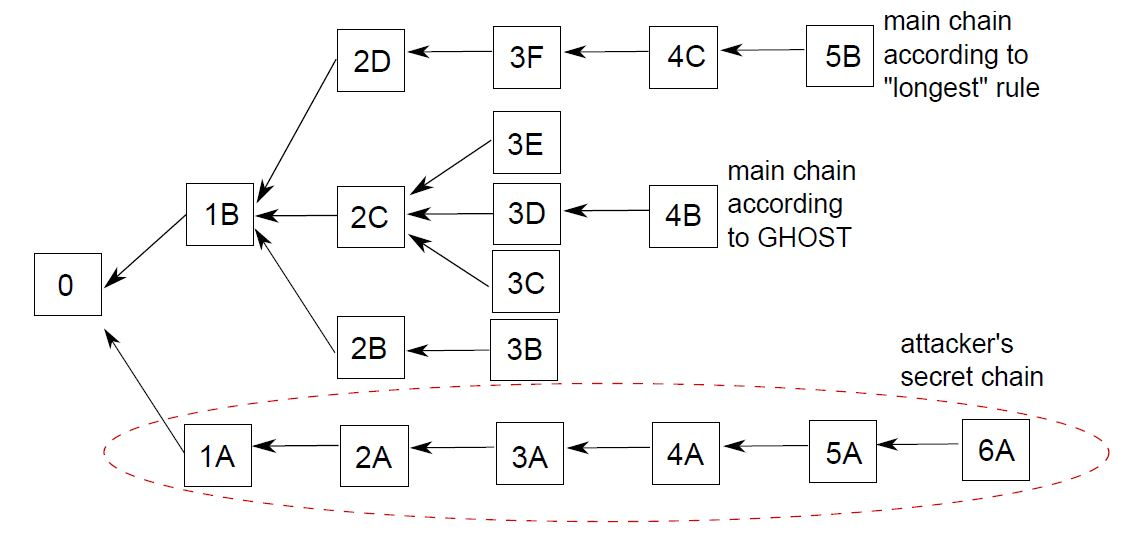
\includegraphics[width=0.8\textwidth,angle=0]{images/forking-risks}
     \caption{Auswahl der gültigen Blockchain. In Bitcoin die längere Blockchain. In Ethereum die Blockchain }
    \label{fig:forking-risks}
\end{figure} 

%Das Problem der Benachteiligung der Miner wird dadurch gelöst, dass es ihnen möglich ist zu entscheiden, ob sie einen neu gefunden Block ignorieren. Mit Bezug zum oberen Beispiel: Miner A, mit 45\% der Rechenleistung, findet einen Block und  alle anderen Nodes erhalten diesen nach 4 Sekunden. Die Wahrscheinlichkeit sehr gering ist, dass sie innerhalb von einer Sekunde einen Block finden welchen sie an den neuen anhängen können. Deshalb entscheiden sich die Nodes dazu den Block zu ignorieren, und arbeiten mit 55\% der Rechenleistung weiter am alten Block. Dies führt dazu, dass sie 

\paragraph{Schlechtere Skalierbarkeit durch Smart Contracts}
%TODO: S.21 Scherer: Sharing Explanation einbauen ?
Ethereum löst die Probleme von häufig auftretenden Forks und erlaubt so einen höheren Transaktionsdurchsatz sowie schnellere Transaktionsbestätigungszeiten. Weitere Probleme entstehen jedoch, wenn eine Blockchain nicht nur Geldtransfertransaktionen verarbeitet. Ethereum erlaubt das speichern und ausführen von eigenem Code durch Smart Contracts. Dadurch steigt die Komplexität der auszuführenden Transaktionen. Dadurch nimmt die Skalierbarkeit ab, da die entstehenden größeren Blöcke eine längere Propagationszeit verursachen. Ebenfalls verschlechtert sich die Performance des Netzwerks, da die Daten schwieriger zu verarbeiten sind. So muss jede Node alle Transaktionen verifizieren, Smart Contract-Code ausführen, und die Ergebnisse speichern. \cite{SchererPerformanceScalabilityBlockchain2017}. 

In Ethereum werden Transaktionen sequentiell bei allen Nodes ausgeführt. Dazu gehört das ausführen von Smart Contract-Code sowie das verifizieren der Ergebnisse. Nur so können in Konflikt stehende Transaktionen, wie zum Beispiel beim Double-Spend) erkannt werden. Eine Parallelausführung ist nicht möglich. Dies verschlechtert letztendlich die Performance des Netzwerks, da es länger dauert Transaktionen auszuführen \cite{SchererPerformanceScalabilityBlockchain2017}. Dies wird auch durch ein Beispiel klar. Ein Angreifer kann DoS-Attacken ausführen, indem er komplex auszuführende Smart Contracts schreiben. Die Ausführung von diesem bei jeder Node führt dazu, dass keine anderen Operationen ausgeführt werden können. Ethereum löst dieses Problem, indem der Transaktionssender für jeden Berechnungschritt eine Gebühr zahlen muss. Dies funktioniert jedoch nur, wenn in der Blockchain-Anwendung eine Kryptowährung genutzt wird \cite{VukolicRethinkingPermissionedBlockchains2017}. 

%TODO: Wenn mehrere Authoren: Alle erwähnen ?
Ebenfalls behauptet Vukolic, dass der Code der Smart Contracts nicht bei allen Nodes ausgeführt werden muss. Um Konsens zu erreichen genügt es, dass alle Nodes den gleichen Stand der Daten erhalten. Deshalb könnte die Codeausführung von nur von bestimmten Nodes ausgeführt werden. Das Problem dabei ist, dass man eine genügend große Anzahl an vertrauenswürdige Teilnehmer festlegen muss \cite{VukolicRethinkingPermissionedBlockchains2017}. Damit geht allerdings auch das vertrauenslose Modell der Blockchain verloren.

%TODO: Lightning Network ?
%TODO: Weiterführende Quellen für Netzwerktopologien ?
%TODO: Bearbeiten, wenn vorheriges Kapitel fertig
Letztendlich lässt sich sagen, dass Public Blockchains nicht skalieren. Um dies zu lösen, müsste die Netzwerktopologie verbessert werden um schnelle Blockpropagrationszeiten zu erlauben \cite{SchererPerformanceScalabilityBlockchain2017}. Weitere Schwierigkeiten bestehen sobald nicht nur Geldtransferaktionen verarbeitet werden müssen. Betrachtet man das CAP-Theorem wird ersichtlich, dass nur die Eigenschaften Dezentralisierung und Sicherheit gegeben sind. Es ist jedoch zu bedenken, dass viele Probleme der Skalierbarkeit aufgrund der genutzten Konsensmechanik bestehen. Auch wenn es teilweise Lösungsvorschläge für diese gibt, genügen sie bisher nicht um Skalierbarkeit herzustellen. Deshalb gilt es, die Limitationen von Permissioned Blockchains sowie alternative Konsensmechaniken für diese zu analysieren.

%TODO: S.23 Scherer: "The bottom line is that public networks are not efficient"
%TODO: MinPermissioned: Introduces a concept for better throughput, but it is not tested (??)
%TODO: S.1-6 LiScalable: Introducing a concept with sattelite chains
%TODO: S.2 LiScalable: Blockchain Sharding Solutions ?

\subsection{Permissioned Blockchains}
%TODO: Governing authority erwähnen ?
Permissioned Blockchains werden eingesetzt, wenn nur bestimmte Teilnehmer an der Blockchain teilnehmen sollen.  Dadurch entsteht eine stärkere Zentralisierung als bei Public Blockchains. Bezieht man sich auf das CAP-Theorem, müssten sich dadurch die Sicherheit und/oder Skalierbarkeit verbessern. Dies führt allerdings auch dazu, dass ein größeres Maß an Vertrauen zwischen den Teilnehmern gegeben sein muss. Dies wird dadurch sichergestellt, dass jeder Teilnehmer die Rechte zur Teilnahme am Netzwerk erhalten hat und die Identitäten dieser bekannt sind. Duch letzteres ist nachverfolgbar, welche Teilnehmer welche Transaktionen ausführt \cite{SchererPerformanceScalabilityBlockchain2017}.

%TODO: Die Analyse erfolgt anhand von Hyperledger Fabric, weil... ?
Scherer behauptet, dass das größere Vertrauen es erlaubt den Nodes verschiedene Aufgaben zuzuteilen. Dies beschreibt er am Beispiel von Hyperledger Fabric, einer Permissioned-Blockchain. In dieser gibt es Peer und Ordering Nodes. Erstere simulieren das ausführen von der Transaktionen und der damit verbundenen Datenänderungen. Letztere bestimmen die Reihenfolge der auszuführenden Transaktionen in den Blöcken. Peer Nodes führen die bereits simulierten Transaktionen nacheinander aus und erkennen Konflikte in den Transaktionen (Genauer im Kapitel \ref{sec:hyperledger-fabric-composer} erklärt). Die Ordering Nodes sind also letztendlich für den Konsens verantwortlich. In Gegensatz zu Ethereum können Peer Nodes so parallel Transaktionen verarbeiten. Sie müssen sich nicht um eventuelle Konflikte oder die Reihenfolge der Transaktionen kümmern. Letztendlich würde die Skalierbarkeit, im Rahmen des Verarbeitens von Transaktionen, von der Hardware der Peers und der Anzahl dieser abhängen. Letzteres würde zu schlechterer Performance führen, da mehr Kommunikation zwischen den Nodes notwendig ist \cite{SchererPerformanceScalabilityBlockchain2017}.

%TODO: Paper mit Transaktionswerten
%TODO: Warum müssen die Endorser kommunizieren
Scherer führt ebenfalls Tests durch um die Performance von Hyperledger Fabric zu analysieren. Dazu nutzt er eine frühe und unstabile Version 1.0. Das Netzwerk besteht aus einer Ordering und einer Peer Node. Es wird kein Konsensmechanismus genutzt. Die Anwendung selber unterstützt die Zahlung mittels digitaler Assets (z.B. Tokens bzw. Coins) zwischen 2 Accounts. Dabei erreicht er einen maximalen Transaktionsdurchsatz von 350 TPS. Dabei ist allerdings zu bedenken, dass der Test auf einer Maschine mit limitierten Ressourcen ausgeführt wird. Um einen maximalen Transaktionsdurchsatz zu erreichen, müssten mehrere leistungsstarke Computer für den Test eingesetzt werden. Scherer stellt ebenfalls fest, dass der Transaktionsdurchsatz abnimmt, desto mehr Peers es gibt, welche Transaktionen bestätigen. Dies liegt daran, dass diese sogenannten Endorser untereinander kommunizieren müssen. Pro Node müssten O(n$^2$) Nachrichten gesendet werden, wobei n die Anzahl an Nodes ist. Die Anzahl an effizient nutzbaren Endorsern ist also beschränkt. Auch hier ist jedoch zu bedenken, dass ein Test mit leistungsstarken Computern ausgeführt werden muss um die Skalierbarkeit dieser festzustellen \cite{SchererPerformanceScalabilityBlockchain2017}.

Ein Paper von Pongnumkul vergleicht die Leistung von Hyperledger Fabric mit Ethereum. Er nutzt dazu die stabile Version 0.6. Er führt die Test ebenfalls mit nur einer Peer Node durch. Zur Ordering Node macht er keine Angabe. Die Anwendung ist die gleiche wie bei Scherer und es wird ebenfalls kein Konsensmechanismus genutzt. Pongnumkul stellt fest, dass die Performance von Fabric in allen Kriterien besser ist als bei Ethereum. So betrug die Zeit, bis eine Beispieltransaktion verarbeitet wurde bei Ethereum 41 Sekunden und bei Ethereum 478 Sekunden. Tests zum maximalen Transaktionsdurchsatz haben ergeben, dass Ethereum 40 TPS und Hyperledger Fabric 300 TPS erreicht hat. Die dazugehörige Abbildung \ref{fig:tps-ethereum-vs-hyperledger} zeigt auch, dass die Unterschiede zwischen Ethereum und Fabric signifikanter sind, desto mehr Transaktionen verarbeitet werden müssen \cite{PongnumkulPerformanceAnalysisPrivate2017}.

\begin{figure}[htb]
  \centering
    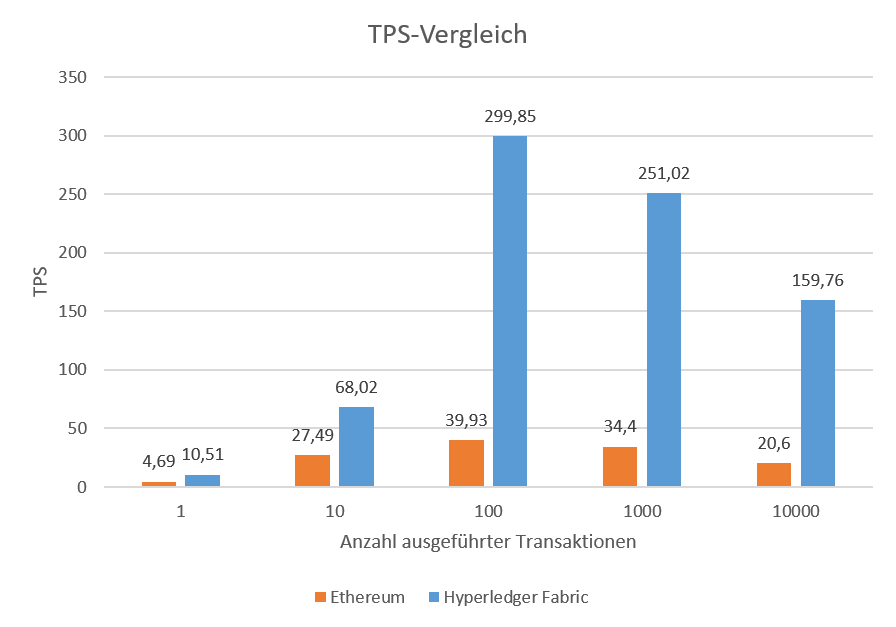
\includegraphics[width=0.8\textwidth,angle=0]{images/tps-ethvshyp}
     \caption{Vergleich des Transaktionsdurchsatzes von Ethereum und Hyperledger Fabric \cite{PongnumkulPerformanceAnalysisPrivate2017}.}
    \label{fig:tps-ethereum-vs-hyperledger}
\end{figure} 

Bei beiden Tests ist zu bedenken, dass sie mit nicht aktuellen Versionen von Hyperledger Fabric ausgeführt wurden. Mittlerweile gibt es eine stabile Version 1.0, sowie eine Preview von Version 1.1.0 \cite{HyperledgerFabricTeamHyperledgerFabricReleases2018}. Es ist also möglich das die Performance sich mittlerweile verbessert hat.

Letztendlich lässt sich sagen, dass Permissioned Blockchains, was die Verarbeitung von Transaktionen betrifft, eine bessere Performance erzielen. Damit bestätigt sich auch das CAP-Theorem bezüglich der Skalierbarkeit. Die Performance wurde allerdings noch nicht unter der Nutzung verschiedener Konsensmechanismen betrachtet. Weiterhin muss das CAP-Theorem noch auf die Sicherheit untersucht werden. Deshalb erfolgt im nächsten Kapitel die Analyse der Skalierbarkeit und Sicherheit von Konsensmechanismen.

%TODO: Am Ende Bezug zum CAP-Theorem ?
\section{Konsensmechanismen}
\label{sec:eval-konsens}
%TODO: Absatz früher nennen ? In den Grundlagen ?
Das Erreichen von Konsens in einer Blockchain, ist eine Abwandlung des Byzantine Generals Problem. In diesem gibt es Generäle, welche Armeen kommandieren welche eine Stadt umzingeln. Ein Angriff auf diese ist nur erfolgreich, wenn alle Armeen gleichzeitig angreifen. Die Generäle müssen untereinander kommunizieren und Konsens darüber herstellen, ob ein Angriff erfolgen soll. Allerdings gibt es Verräter unter diesen. Es handelt sich also um ein vertrauensloses Umfeld. Genau so kann es in einer Blockchain zu den sogenannten Byzantine Faults kommen, wenn nicht vertrauenswürdige Nodes Daten manipulieren können. Deshalb müssen verteilte Systeme Byzantine Fault Tolerance (BFT) herstellen, um eine gewisse Anzahl an nicht vertrauenswürdigen Teilnehmern zu tolerieren. Dies geschieht in Blockchains über die Konsensmechanismen \cite{ZhengBlockchainChallengesOpportunities2017}.

Eine Blockchain, welche den PoW als Konsensmechanismus nutzt, ist nicht skalierbar. Ebenfalls würde er in Netzwerken mit relativ wenig Teilnehmern die Sicherheit beeinträchtigen, da ein Teilnehmer einfacher 51\% der Rechenleistung erreichen kann. Für Permissioned Blockchains muss also ein Konsensmechanismus gefunden werden, welche Skalierbarkeit und Sicherheit herstellt. Aufgrund des höheren Vertrauens in Permissioned Blockchains, behauptet Scherer, dass ein Konsensmechanismus genutzt werden kann, welcher Vertrauen in geringerem Maße als der PoW garantiert. Somit könnten Skalierbarkeit und Sicherheit hergestellt werden \cite{SchererPerformanceScalabilityBlockchain2017}. Im folgenden werden verschiedene Konsensmechanismen verschiedener Blockchain-Technologien miteinander verglichen. Dabei ist zu bedenken, dass nur auf die Konsensmechanismen, welche Sicherheit und Skalierbarkeit in Permissioned Blockchains sicherstellen können, im Detail eingegangen wird.

%TODO: Add Raft/Kafka ?
\subsection{Proof of Stake}
Beim PoS hängt die Wahrscheinlichkeit, einen Block zu minen, von der Menge des Eigentums (z.B. Kryptowährung) eines Nutzers ab. Desto mehr Bitcoins man beispielsweise hat, desto höher ist die Wahrscheinlichkeit für das Mining ausgewählt zu werden. Ähnlich wie beim PoW könnte ein Teilnehmer mit 51\% aller Bitcoins das Netzwerk angreifen, da er die längere Blockchain erstellen kann. Aber selbst wenn es ein Teilnehmer schafft, 51\% der Bitcoins zu besitzen, hätte er keine Motivation dazu. Denn letztendlich würde ein Angriff den Kurs von Bitcoin senken, und somit würde der Miner sich selber schaden \cite{ZhengBlockchainChallengesOpportunities2017}. Da der PoS hauptsächlich nur bei Kryptowährungen genutzt werden kann, ist er für Permissioned Blockchains uninteressant.

\subsection{Proof of Elapsed Time}
Der PoET wird in Intels Blockchain-Technologie Hyperledger Sawtooth genutzt. Die grundlegende Idee ist, dass eine Node eine zufällige Zeit generiert, welche Sie warten muss um einen Block zu erstellen. Um sicherzustellen, dass die generierte Zeit nicht verfälscht wurde, wird Trusted Computing \footnote{Trusted Computing: Soft- und Hardware stellen sicher, dass ein Computer sich wie erwartet verhält \cite{WikipediaTrustedComputing2018}} genutzt. So stellen Intels Software Guard Extensions (SGX) sicher, dass Code nicht modifiziert werden kann. Eine Node muss also über solchen unmodifizierbaren Code eine Zeit generieren. Weiterhin erfolgen statistische Tests, um zu verhindern dass eine Node Blöcke zu schnell und somit zu oft erstellt. Letztendlich ist die Blockerstellung damit fair verteilt, und kein Teilnehmer kann die Blockchain kontrollieren. Im Prinzip funktioniert der Mechanismus wie der PoW. Dort wird eine Wartezeit durch das Finden eines Hashes sichergestellt, während dies beim PoET durch die Hardware sichergestellt wird. Dadurch, dass es keine rechenintensiven Aufgaben gibt, ist die Skalierbarkeit sicher gestellt. Es ist jedoch zu bedenken, dass es bisher wenige Analysen zu der Sicherheit des PoET gibt. Ein Paper von Chen stellt fest das der Konsensmechanismus unter bestimmten Umständen unsicher ist, schlägt aber auch Lösungen dafür vor. Ebenfalls kommt hinzu, dass man der Hardware von Intel für das Trusted Computing vertrauen muss. \cite{ChenSecurityAnalysisProofofElapsedTime2017}.

%TODO: Erwähnen bei welchen Mechanismen die Teilnehmer bekannt sein müssen ?
%TODO: Skalierbarkeit genauer auf Transaktionsdurchsatz und Anzahl an Nodes beziehen ?
\subsection{Diversity Mining Consensus}
Der Diversity Mining Consensus ist ähnlich dem PoW. In diesem ist der Block einer Node nur valide, wenn sie eine bestimmte Anzahl an vorherigen Blöcken nicht erstellt hat. Dies führt letztendlich dazu, dass eine Wartezeit für jede Node nicht durch das Finden eines Hashes (Siehe PoW) oder durch eine generierte Zeit (Siehe PoET) realisiert wird. Auch hier kann es zu Forks kommen, wenn 2 Nodes zur ungefähr gleichen Zeit einen Block erstellen. Ebenfalls wird die entstehende längere Blockchain akzeptiert. Durch die Wartezeit wird sichergestellt, dass der Branch mit den meisten Minern die längere Blockchain erstellt. Die Gefahr bei diesen Konsensmechanismus ist, dass bösartige Miner sich zusammen tun können. Unter den richtigen Umständen erstellt der Zusammenschluss die meisten Blöcke, und kann somit auch bei Forks eine längere Blockchain erstellen, um so Double-Spend-Angriffe auszuführen. Die Skalierbarkeit ist aufgrund des fehlenden Rechenaufwands gegeben. \cite{GreenspanMultiChainPrivateBlockchain2015}\cite{CachinBlockchainConsensusProtocols2017}.

%TODO: Weglassen ?
\subsection{QuorumChain}
Quorum ist ein Fork von Ethereum für Permissioned Blockchains. Dieser nutzt den Konsensmechanismus QuorumChain. Es gibt Voter und Block-Maker Nodes. Die Block-Maker schlagen Blöcke zum erstellen vor, und die Voter stimmen für diese ab. Um Forks zu verhindern, warten die Block-Maker eine zufällige Zeit und erstellen den Block. Die Voter validieren diesen und stimmen für ihn ab, indem Sie u.a. die Transaktionen ausführen und überprüfen ob der vorherige Block genug Stimmen erhalten hat. Die Nodes hängen letztendlich den Block an ihre lokale Chain an, welcher einen bestimmten Schwellwert an Stimmen überschritten hat, oder im Falle eines Forks die meisten Stimmen erhalten hat. Die Sicherheit des Mechanismus ist fragwürdig. Schon allein mit einen bösartigen Block-Macker würde es ständig zu Forks kommen, welche Double-Spend-Angriffe ermöglichen und die Zeit erhöhen bis eine Transaktion nicht mehr verworfen werden kann \cite{CachinBlockchainConsensusProtocols2017}.

%TODO: Mehr Details aus Terndermint übernehmen ?
\subsection{Practical Byzantine Fault Tolerance}
Der PBFT gehört zu der Familie der BFT-Protokolle. Beim PBFT wählen die Teilnehmer eine Leader-Node. Jede Runde schlägt diese diese einen neuen Block mit auszuführenden Transaktionen vor. Dieser wird an alle anderen Nodes weitergeleitet. Anschließend wird der Konsens hergestellt. 2/3 der Nodes müssen dem im Block enthaltenen Transaktionen zustimmen, damit er erstellt wird. Erst dann werden die Transaktionen bei jeden Teilnehmer ausgeführt. Deshalb können bis zu 1/3 der Nodes unvertrauenswürdig sein. Ein Angreifer müsste für einen Angriff die Kontrolle über 2/3 der Nodes haben \cite{SukhwaniPerformanceModelingPBFT2017a}\cite{ZhengBlockchainChallengesOpportunities2017}. 

Vukolic behauptet, dass es BFT-Protokolle gibt, welche einen Transaktionsdurchsatz von mehreren 10000 TPS unterstützen. Die Skalierbarkeit dieser bezüglich der Anzahl an Nodes ist jedoch begrenzt \cite{Vukolicquestscalableblockchain2015}. Croman erzielt bei seinen Tests mit dem PBFT, bei 8 Nodes und 8192 auszuführenden Transaktionen einen Transaktionsdurchsatz von 14000 TPS. Weiterhin wird ersichtlich wie die Performance mit der Anzahl an Nodes abnimmt. Mit 64 Nodes und 8192 auszuführenden Transaktionen wird ein Transaktionsdurchsatz von 4500 TPS erreicht \cite{CromanScalingDecentralizedBlockchains2016}. Im Gegensatz zum PoW besteht hier eine bessere Skalierbarkeit bezüglich des Transaktionsdurchsatzes, allerding ist sie bezüglich der Anzahl an Teilnehmern begrenzt \cite{Vukolicquestscalableblockchain2015}.

Ein weiterer Vorteil von BFT-Protokollen ist, dass es Consensus Finality gibt. Das bedeutet, dass es nicht zu Forks kommen kann. Somit müssten Nutzer nicht darauf warten, dass mehrere Blöcke nach einer Transaktion erstellt werden, damit die Sicherheit gegeben ist, dass diese endgültig bestehen wird. Somit entfällt auch die Gefahr von Double-Spend-Attacken \cite{Vukolicquestscalableblockchain2015}.

Die Angriffe, welche mit mehr als 1/3 der Voting Power erfolgen können, sind die sogenannten Censorship Attacks. So könnten Nodes verhindern, dass neue Blöcke entstehen, indem sie ihre Stimme zurückhalten. Weiterhin könnten sie bestimmte Transaktionen zensieren, indem sie dafür stimmen diese nicht in einem Block aufzunehmen \cite{TendermintTeamTendermintGithubRepository2018}.

\subsection{Tendermint}
Tendermint ist eine Abwandlung des PBFT-Konsensmechanismus. Der größte Unterschied besteht darin, dass die Nodes, welche eine Block vorschlagen, in einem Round-Robin Verfahren ausgewählt werden. So gibt es in jeder Runde einen neuen Blockersteller. Hinzu kommt, dass die Teilnehmer mit ihren Coins, welche die Voting Power bestimmen, abstimmen. Die Coins werden für einen Vote für eine bestimmte Zeit an die Vote gebunden und damit für die weitere Nutzung gesperrt. Aufgrund der Asynchronität des Netzwerks kann es passieren, dass eine Node noch keine Information über einen bereits neu erstellten Block erhalten hat. Das führt dazu, dass er einen neuen Block auf der gleichen Höhe des bestehenden Blocks vorschlägt. Es kann dann zu einen Fork kommen, wenn beide Blöcke 2/3 der Voting Power erhalten. Dies ist nur möglich, wenn mindestens 1/3 der Voting Power bösartig genutzt werden. Diese Nodes können jedoch bestraft werden. Durch die an die Abstimmung gebundenen Coins, können Nodes, welche bösartig abgestimmt haben, bestraft werden. So werden die gebundenen Coins einfach zerstört \cite{KwonTendermintConsensusmining2014}\cite{BuchmanTendermintByzantineFault2016}. Es ist zu bedenken, dass Tendermint-Konsensus nur mit einer Kryptowährung im vollen Umfang funktioniert.

\subsection{Sonstige BFT-Konsensmechanismen}
Neben den bisher erwähnten BFT-Konsensmechanismen, gibt es noch diverse andere welche das Prinzip des PBFT mehr oder weniger abwandeln. So gibt es Symbiont und R3 Corda mit BFT-SMaRt, Iroha mit Sumeragi, Kadena mit ScalableBFT und Chain mit Federated Consensus \cite{CachinBlockchainConsensusProtocols2017}. Aufgrund der Vielfalt und Detailreichheit jeder dieser Konsensmechanismen, wird nicht genauer auf sie eingegangen. Es genügt die Prinzipien von BFT-Protokollen anhand des PBFT zu verstehen.

\subsection{Zusammenfassung}
In Permissioned Blockchains bieten sich vor allem Konsensmechanismen an, welche auf BFT-Protokollen beruhen. Diese können je nach genutzten Protokoll Skalierbarkeit und Sicherheit herstellen. Es ist allerdings auch zu bedenken, dass sie weniger Sicherheit als beispielsweise der PoW garantieren. Somit kann letztendlich auch eine Aussage zu den CAP-Theorem getroffen werden. Die geringere Dezentralisierung sowie Sicherheit sorgen für eine höhere Performance, und damit für bessere Skalierbarkeit.

\section{Sonstige Einschränkungen}

%TODO: Consensus with private transactions genauer erklären ?
\subsection{Private Transaktionen}
In Blockchains wie bei Bitcoin und Ethereum ist es nicht möglich, private Transaktionen auszuführen. Das bedeutet, alle Transaktionen sind für alle Teilnehmer sichtbar. In Permissioned Blockchains kann es Fälle geben, wo dies nicht erwünscht ist. So soll z.B. eine Preisabsprache zwischen 2 Teilnehmern in der Blockchain dokumentiert werden, welche für andere nicht sichtbar sein soll.

In Quorum wird dies so realisiert, dass in einer Transaktion angegeben wird, welche Teilnehmer die Transaktion sehen dürfen. Diese wird anschließend verschlüsselt, und kann nur von den angegebenen Teilnehmern entschlüsselt werden. Die Transaktion wird im Netzwerk verteilt, und nur von den Teilhabern ausgeführt \cite{QuorumTeamTransactionProcessingQuorum2018}.

In Hyperledger Fabric werden Private Transaktionen über Channels ermöglicht. Dabei ist jeder Channel eine eigene Blockchain, mit verschiedenen Teilnehmern. So würde es beispielsweise einen öffentlichen Channel geben, an welchen alle Teilnehmer der Permissioned Blockchain teilnehmen. Zusätzlich würde es private Channel geben, welche nur zwischen bestimmten Teilnehmer bestehen würden. Keine Daten können zwischen den Channeln übertragen werden \cite{SchererPerformanceScalabilityBlockchain2017}. 
%TODO: S.2 WustYouNeedBlockchain: Tensio between Transparency and Privacy ?

%TODO: Add Non-Deterministic Execution ?
%\subsection{Code Execution}
%S.2 VukolicRethinking: Non-Deterministic Execution

\subsection{Datenmenge}
Ein noch nicht angesprochenes Problem der Blockchain ist die Datenredundanz im Bezug auf die Datenmenge. Da keine Daten in der Blockchain gelöscht werden können, wächst sie stetig an. So ist die Bitcoin-Blockchain im Moment 151GB groß \cite{BlockchainUnternehmenBlockchainSizeBitcoin}. Größere Datenmengen werden schneller erreicht, wenn nicht nur Geldtransferaktionen bestehen.

Die Datenmenge stellt ein Problem dar, da Teilnehmer ab einen bestimmten Punkt eventuell nicht mehr bereit sind die Blockchain auf ihrer Node zu speichern. Dies würde zu weniger Minern, und somit zu höherer Zentralisierung führen \cite{SchererPerformanceScalabilityBlockchain2017}.

%TODO: Zusammenfassung zu den Kapitel ?





